\documentclass[../lecture.tex]{subfiles}

\begin{document}

\correction{rdm-0022}

\fincorrection

\end{document}

\begin{enumerate}
  \item coming

  \item \

  \begin{center}
    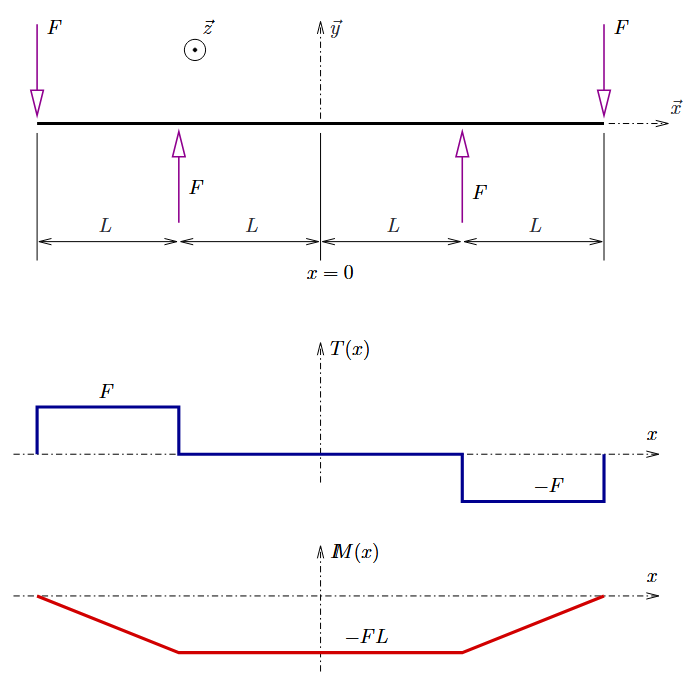
\includegraphics[scale=0.6]{figB0022.png}
  \end{center}

  \item La contrainte maximum est :
  $$
  \sigma_{\text {Max }}=\frac{F L}{I} \frac{h}{2}=\frac{12 F L h}{b h^{3}} \frac{6 F L}{2}=\frac{6 F^{2}}{b h^{2}}=160 \mathrm{MPa}
  $$
  Cette contrainte est en compression pour $y=-\frac{h}{2}$ et en traction pour $y=+\frac{h}{2}$. Le coefficient de sécurité vaut $2.81 .$


  \item Pour $x \in[0: L]$ on a
  $$E I v^{\prime\prime} = - FL$$
  en intégrant une prmière fois on a alors
  $$E I v^{\prime}=-F(Lx + A)$$
  où $A$ est une constante. Puis en intégrant une seconde fois on obtient
  $$E I v=-F\left(L \frac{x^{2}}{2}+A x+C\right)$$
  où $C$ est une constante.

$$
\begin{array}{r}
x \in[L: 2 L] \\
E I v^{\prime \prime}=F(x-2 L) \\
E I v^{\prime}=F\left(\frac{x^{2}}{2}-2 L x+B\right) \\
E I v=F\left(\frac{x^{3}}{6}-2 L \frac{x^{2}}{2}+B x+D\right)
\end{array}
$$

La symétrie du problème fait que $v^{\prime}(0)=0 \quad \Longrightarrow \quad A=0$.
De plus nous devons avoir $v(x)$ et $v^{\prime}(x)$ continues en $x=L$ et $v(L)=0$ pour les 2 expressions ce qui s'écrit :

$$
\begin{gathered}
-\left(L^{2}\right)=\left(\frac{L^{2}}{2}-2 L^{2}+B\right) \quad \Longrightarrow \quad B=\frac{L^{2}}{2} \\
L \frac{L^{2}}{2}+C=0 \quad \Longrightarrow \quad C=-\frac{L^{3}}{2} \\
\frac{L^{3}}{6}-2 L \frac{L^{2}}{2}+B L+D=0 \quad \Longrightarrow \quad \frac{L^{3}}{6}-\frac{6 L^{3}}{6}+\frac{L^{3}}{2}+D=0 \quad \Longrightarrow \quad D=\frac{L^{3}}{3}
\end{gathered}
$$


On obtient alors:

$$
\begin{array}{r}
x \in[0: L], X=\frac{x}{L} \in[0: 1] \\
E \operatorname{Iv}(x)=-F\left(L \frac{x^{2}}{2}-\frac{L^{3}}{2}\right) \\
E I v(X)=\frac{F L^{3}}{6} \underbrace{\left(-3 X^{2}+3\right)}_{f(X)}
\end{array}
$$

$$
\begin{array}{r}
x \in[L: 2 L], X=\frac{x}{L} \in[1: 2] \\
E I v(x)=F\left(\frac{x^{3}}{6}-2 L \frac{x^{2}}{2}+\frac{L^{2}}{2} x+\frac{L^{3}}{3}\right) \\
E I v(x)=\frac{F L^{3}}{6} \underbrace{\left(X^{3}-6 X^{2}+3 X+2\right)}_{g(X)}
\end{array}
$$


Le tracé des 2 courbes adimensionnées donne l'allure de la déformée amplifiée par 20 environ :



\begin{center}
  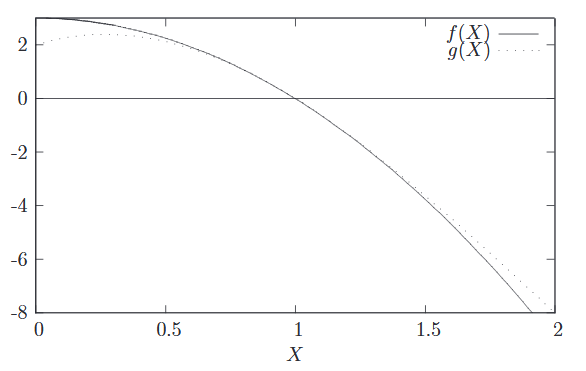
\includegraphics[scale=0.6]{figC0022.png}
\end{center}



La flèche maximum est $|v(2 L)|=8 \frac{F L^{3}}{6 E I}=\frac{4 F L^{3}}{3 E I}=16.25 \mathrm{~mm}$.
Le moment est extrème sur tout $x \in[-L: L]$ et vaut $-F L=-320$ N.m.

\end{enumerate}
